\section{Implementation}
\label{sec:implementation}

\subsection{Overview}

To meet the performance requirements of the data center, we implemented \OurSys
on the Xilinx Zynq UltraScale+ MPSoC ZCU102 Evaluation Kit.  This platform is
powered by a ZU9EG System-on-Chip FPGA consisting of a quad-core ARM Cortex-A53, a
dual-core ARM Cortex-R5, and a programmable fabric with 274K lookup tables
(LUTs) and 1800 18Kb embedded memories (BRAMs).
% I guess we need to introduce FPGA more for a network audience...
% Why did we choose to implement on FPGA?
%   Support by example of network paper that performs well on FPGA?

\begin{figure}
  \centering
  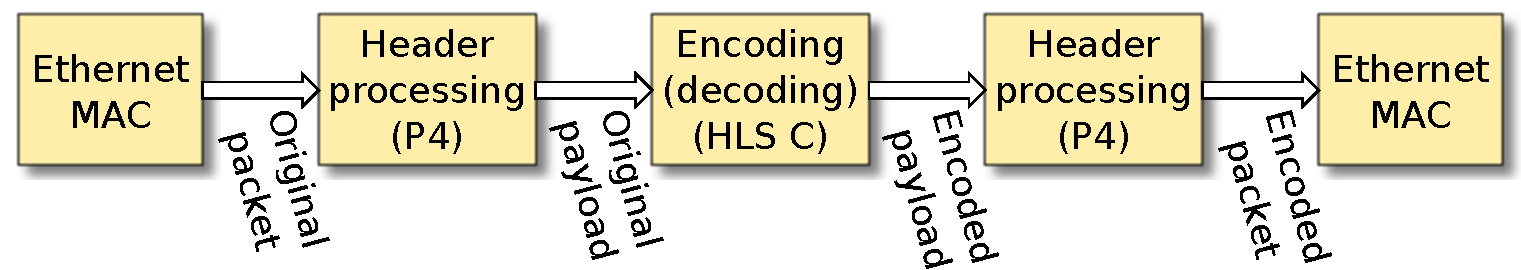
\includegraphics[width=0.4\paperwidth]{Top_level.pdf}
  \caption{\label{fig:toplevel} Block diagram of encoder / decoder pipeline}
\end{figure}

A top-level diagram of the implementation is shown in Fig.~\ref{fig:toplevel}.
Packets arrive on one of the 4 SFP+ cages via a 10Gbps Ethernet cable.
A dedicated 10~Gigabit Transceiver deserializes the packets.  After further
processing by a dedicated Ethernet PHY and in-fabric MAC layer, the entire
packet including Ethernet header is output on a 64-bit AXI Stream bus at 160\,MHz.

The next stage in the pipeline performs packet header preprocessing.  With
ease of implementation and portability in mind, we implemented this in P4, a
domain-specific programming language for packet processing that is target- and
protocol-agnostic \cite{p4_sigcomm_review2014}.  The raw payload, i.e. the frame stripped of Ethernet
header, is forwarded to the FEC core.  \amdrev{The P4 is compiled to FPGA
  logic using Xilinx's SDNet tool suite.}

The FEC core can be an encoder (for the Sending Proxy) or decoder (for the
Receiving Proxy).  In both cases, the FEC core
produces payloads that are the result of, respectively, encoding or decoding
the received group of payloads.  Similar to the header processing, the FEC core
was also created with ease of implementation in mind.  P4 is not suitable
for
\amdrev{payload processing or}
exploiting the parallellism of the FEC core, so we described the core in
hardware-synthesizable C.  As usual, the code can be compiled and executed on a
general-purpose CPU.  More importantly, we can synthesize the code for an FPGA
in Vivado HLS.  Guided by pragmas added by the developer, Vivado HLS takes
advantage of parallelism in the code to achieve a high performance.

The encoded or decoded output of the FEC core feeds into the header
post-processing, which encapsulates the payloads in Ethernet packets.  The
Ethernet subsystem, finally, returns the packets to the network.

\subsection{Header processing}

We use p4 to implement high-level packet processing logic and 

use Xilinx P4-SDNet tool chain to translate p4 program into FPGA and integrate everything together

The translation goes through 3 steps:

First, from P4 to SDNet

Second, from sdnet to RTL implementaion and C++ high-level simulation

Third, add prepheral blocks with Vivado Design Suit

what does P4 do?
Parse packet, modify and tag headers as is described in Design chapter, extract payload for encoder,
control encoder's operation

what is SDNet?
intermediate language, describes the interface, layout, and data flow of data processing engines
at a level closer to RTL modules compared to P4.

\amd{not sure what value the above has -- I do suggest hoisting the SDNet
  comment into the previous section}

%introduce RTL/FPGA?

several challenges:
1. Both P4 and SDNet encourage programs working like a flow - you should never go back and touch anything
a second time. This ensures the efficiency of the program but also makes it harder to express complex
logics. We think it can be a future work to translate a loosely written program into one with such constrains.
Currently we do this manually by keeping in mind a dependency graph of program lines and doing a topological sort
to decide the final order. Using compound operations like
$read\_and\_add\_one$ also helps mitigating this problem.
\amd{I am not following this...and I doubt a reader with no knowledge of
  FPGAs or SDNet will be able to follow either.  What does ``go back'' mean
  in this context? What are you ordering? How is the read-and-add-one
  addressing the problem?}

2. P4 is designed particularly for header processing. There are many
irrelevant \amd{irrelevant is probably not the right word here} things not supported but
necessary in our work, especially payload processing. Most bookkeeping operations can be finished with the
help of external functions like $read\_and\_add\_one$, later implemented in C or Verilog. We also integrate the encoder
into the design by defining an external function for it. However, encoding payload through this interface can be a
great waste for both time and space due to P4's nature of passing and processing a packet as a whole, no matter how long it is. Fortunately, the
flexibility we seek can be found by redirecting SDNet's internal packet flow, which works similar to a 64-bit AXI Stream bus,
to the engine for encoder. This involves modification of less than 10 lines of code per SDNet program, and can be finished by a simple script.
\amd{...don't think this works for a reader either...  Yes, we want to make
the case that P4 doesn't allow payload processing (I suggest adding a note
about that above).  Do we want to dig into the fact that P4 doesn't give us
the expressiveness to stream payload processing, but SDNet does?  ... if
so, we'll need to setup the problem better here and be clearer about the
shape of the solution.}

\subsection{FEC Encoder}

The current implementation is limited to packet encoding, but our intention is
to implement the decoder, too.

Error correction is performed with a Reed-Solomon erasure (RSE) code.  Erasure codes
require prior knowledge of which packets data is missing, as opposed to regular
error correction codes.  This comes with the benefit of requiring fewer error
correction bits.  RSE is a linear code, which means...

\amd{what do we want to highlight here?
  (1) data parallel nature of way FEC RSE is defined ... allows operate on
  the 8 bytes in the 64b per cycle payload independently in data-parallel
  fashion.
  (2) as k scales up, demands more compute...which can address with more
  hardware.
  (3) result is can build hardware to process in a spatial pipeline at the
  160\,MHz data rate necessary to meet 10Gbps link.
  (4) maybe sketch out how much hardware is needed (8$\times$(2+1)$\times$k
  BRAMs)
}

\begin{comment}
Introduce P4.
- Advantages of writing in high-level languages.
- Responsibilities of P4.
- Communication between P4 and encoder
Implementation process
- SDNet
- Vivado HLS
- Vivado
Introduce FPGA.
Top-level design
Matrix multiplication
\end{comment}

